\documentclass{budisicposter}

\addbibresource{bibliography.bib} % bibliography file

% Title, Author, Institute
\title{A most excellent research project}
\author{First Author$^1$, Second Author$^2$}
\institute{${}^1$ Clarkson, ${}^2$ Not Clarkson}


 \begin{document}

\maketitle

 \begin{columns}%blocks will be placed into columns
       \column{.33}
       \block{Title}{
         Math:
         \[
           \int_0^t f(x(\tau))d\tau
         \]

         We can also put a graph in and refer to it here: Fig.~\ref{fig:first}
         \begin{tikzfigure}[This is a graph.]\label{fig:first}
           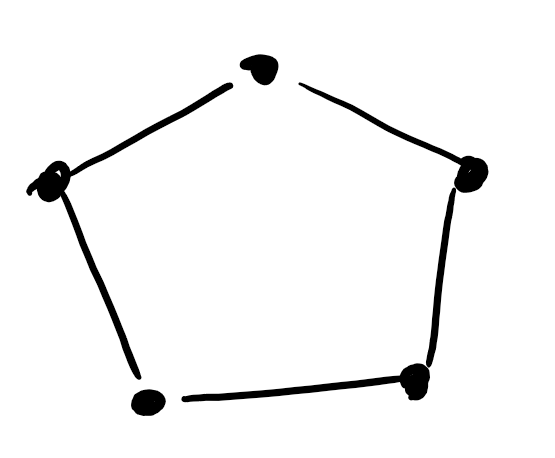
\includegraphics[width=0.5\linewidth]{figs/graph}
         \end{tikzfigure}
       }
       \column{.33}
       \block{Methods}{
         Something common.
         \coloredbox{Important statement can be highlighted}
       }
       \begin{subcolumns}
         \subcolumn{.5}
         \block{Type 1}{
           Something cited from
           \cite{Hill1894}
         }
         \subcolumn{.5}
         \block{Type 2}{
           Something else}
       \end{subcolumns}
       \block{More}{
         For more information, take a look at \texttt{tikzposter-example.tex} and \texttt{tikzposter-example.pdf} in this folder.
       }
       \note[targetoffsetx=2in, angle=-45,targetoffsety=0in,connection]{Additionally, documentation for the poster class is in \url{https://ctan.org/pkg/tikzposter}.}


       \column{.33}

       \block{Results}{
Most people get matrices wrong (overly complicated) in \LaTeX. This is the right way:
\[ %this produces unenumerated equation.
  \begin{bmatrix}
    1 & 2y \\
    \ast & 3x
  \end{bmatrix}
\]



\begin{tikzfigure}[Title]
   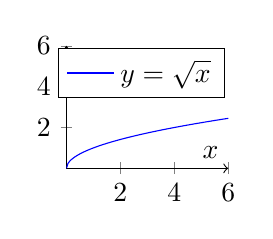
\begin{tikzpicture}
     \begin{axis}[
       xmin=0, xmax=6,
       xlabel={$x$},
       ymin=0, ymax=6,
       ylabel={$y$},
       axis lines=middle,
       axis line style=->,
       width=.3\linewidth]
        \addplot[no marks,blue,-,domain=0:6, samples=100] expression{sqrt(x)};
        \addlegendentry{$y=\sqrt{x}$};
      \end{axis}
   \end{tikzpicture}
 \end{tikzfigure}

 On posters, adding annotations to graphs is a very effective way to communicate what is displayed AND at the same time reduce the amount of text. For more annotation examples, see the end of the document

      \draw[arrow,->] (15,8) % head of arrow (notice the arrow symbol after \draw command)
     -- node [text width=1.5in,midway,above,left] {Annotation 3}
     +(45:8); % 45 degrees, length = 8

}

       \block{References}{
         \printbibliography[heading=none]
       }

     \end{columns}

%% Annotations
% default styles for "arrow" and "bubble" are defined just above "\begin{document}"
% search for commands \tikzstyle
%
%  On posters, adding annotations to graphs is a very effective way to communicate
%  what is displayed AND at the same time reduce the amount of text. For more
%  annotation examples, see the end of the document

     \draw[arrow,<->] (12,11) % tail of arrow
     node[bubble] {Annotation 1} % annotation text
     -- % line
     +(-150:3); % tip of arrow: angle 135, length=2

     \draw[arrow] (10,-16) %anchor point - experiment to see how the coordinates move
     -- % line
     +(45:3) % arrow leaves the anchor at 45 degrees and continues for 3 units
     node[bubble, text width=3in] {Annotation Example: See end of LaTeX document}; % annotation text



 \end{document}




\endinput
%%
%% End of file `tikzposter-example.tex'.
